%{{{ Formatierung

\documentclass[a4paper,10pt]{article}

\usepackage{physics_notetaking}

%%% dark red
%\definecolor{bg}{RGB}{60,47,47}
%\definecolor{fg}{RGB}{255,244,230}
%%% space grey
%\definecolor{bg}{RGB}{46,52,64}
%\definecolor{fg}{RGB}{216,222,233}
%%% purple
%\definecolor{bg}{RGB}{69,0,128}
%\definecolor{fg}{RGB}{237,237,222}
%\pagecolor{bg}
%\color{fg}

\newcommand{\td}{\,\text{d}}
\newcommand{\RN}[1]{\uppercase\expandafter{\romannumeral#1}}
\newcommand{\zz}{\mathrm{Z\kern-.3em\raise-0.5ex\hbox{Z} }}
\newcommand{\id}{1\kern-.258em1}

\newcommand\inlineeqno{\stepcounter{equation}\ {(\theequation)}}
\newcommand\inlineeqnoa{(\theequation.\text{a})}
\newcommand\inlineeqnob{(\theequation.\text{b})}
\newcommand\inlineeqnoc{(\theequation.\text{c})}

\newcommand\inlineeqnowo{\stepcounter{equation}\ {(\theequation)}}
\newcommand\inlineeqnowoa{\theequation.\text{a}}
\newcommand\inlineeqnowob{\theequation.\text{b}}
\newcommand\inlineeqnowoc{\theequation.\text{c}}

\renewcommand{\refname}{Source}
\renewcommand{\sfdefault}{phv}
%\renewcommand*\contentsname{Contents}

\newenvironment{Figure}
  {\par\medskip\noindent\minipage{\linewidth}}
  {\endminipage\par\medskip} % for multicols figures

\pagestyle{fancy}

\sloppy

\numberwithin{equation}{section}

%}}}

\begin{document}

%{{{ Titelseite

\begin{titlepage}
        \title{3/4 (2. Halbtag) $|$ Transistor und Transistorverstärker}
        \author[1]{Angelo Brade\thanks{s72abrad@uni-bonn.de}}
        \author[1]{Jonas Wortmann\thanks{s02jwort@uni-bonn.de}}
        \affil[1]{Rheinische Friedrich--Wilhelms--Universität Bonn}
        \date{\today}
\end{titlepage}

\maketitle
\pagenumbering{gobble}

%}}}

\clearpage

%{{{ Inhaltsverzeichnis

\fancyhead[R]{\leftmark}
%\fancyhead[R]{\leftmark\\\rightmark}
\fancyhead[L]{\thepage}
\fancyfoot[C]{}

\tableofcontents

%}}}

\clearpage

%{{{

\pagenumbering{arabic}

\begin{multicols}{2}
        \sloppy
        \section{Introduction}
        In this experiment, the bipolar transistor is used, but here as an emitter sequence for voltage amplification and as an impedance converter.
        Also, the negative feedback of alternating current and the behavior of different frequencies will be observed via a cascode circuit.

        \section{Theory}
        Still the whole theory of different kinds of transistors is needed.
        An emitter follower is an elektronic component, with which a current can be amplified (factor $\gamma $), without any change in voltage (factor $v$).
        \begin{align} 
                v &= \diff[]{U_E}{U_B}\approx 1 & \gamma &= \diff[]{I_E}{I_B}\approx 100
        .\end{align} 
        This is why sometimes an emitterfollower is called an impedance changer.
        \\\\ The negative feedback factor $k$ denotes, which fraction of the output voltage is 
        \begin{align} 
                \dfrac{1}{v} &= \dfrac{1}{v_0}+k
        .\end{align} 
        Die Verstärkung mit Gegenkopplung $v$ ist hier zwar kleiner als die Leerlaufverstärkung $v_0$, allerdings hängt diese nur noch von der äußeren Beschaltungen und nicht mehr von $v_0$, also dem Transistor, ab.
        Diese Verstärkung kann man beschreiben wie
        \begin{align} 
                \dfrac{\td v}{v} &= \dfrac{\td v_0}{v_0}\dfrac{v}{v_0}
        .\end{align} 
        \\Die Bandbreite einer Verstärkerschaltung ist der Frequenzbereich, innerhalb dessen die Verstärkung konstant ist.
        Für die Erhöhung der Bandbreite wird eine Kaskodenschaltung verwendet.
        Um solch eine Vergrößerung zu erzielen wird die wechselspannungsmäßige Rückkopplung des Kollektors auf die Basis verringert, indem ein großer Spannungshub durch die Verwendung eines zweiten Transistors vermieden wird.
        Existiert nun ein Eingangssignal, so ist die daraus resultierende Spannungsänderung im Spannungshub viel geringer als die Änderung der Ausgangsspannung.
        Dadurch ist die Bandbreite einer solchen Kaskodenschaltung größer.
        \\\\Arbeitspunktstabilisierung kann mit Hilfe von Gegenkopplung erzielt werden.
        Eine Möglichkeit dafür ist die Spannungsgegenkopplung.
        \begin{figure}[h]
                \centering
                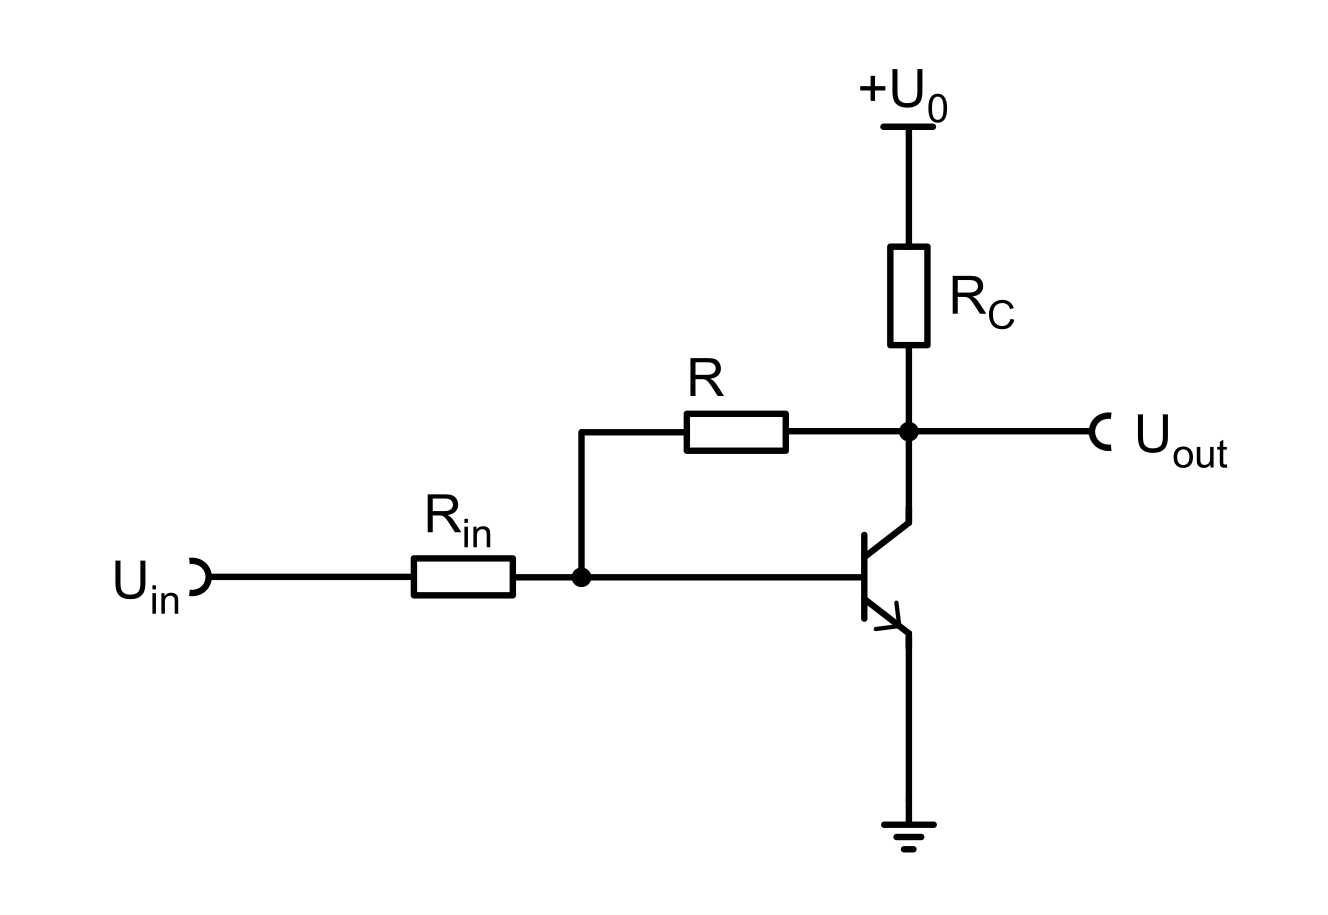
\includegraphics[width=0.6\textwidth]{spannungsgegenkopplung.png}
                \caption{Transistorverstärker in Emitterschaltung mit Spannungsgegenkopplung; Abbildung 2/4.16 \cite{Praktikumsanleitung}}
                \vspace{100cm}
        \end{figure}\\
        Hier stellt der Wiederstand $R$ das Basispotential und damit den Arbeitspunkt ein und er koppelt die Spannung am Kollektor zurück zur Basis.
        Durch diese Gegenkopplung verkleinert sich der Basisstrom bei konstanter Eingangsspannung.

        \newpage
        \section{Preliminary Tasks}
        \subsection{G}
        $\zz\ v=\tfrac{\gamma R_E}{r_{BE}+\gamma R_E}$ mit $\gamma =\diff[]{I_E}{I_B}$ und $r_{BE}=\diff[]{U_{BE}}{I_B}$.
        \begin{align} 
                && v &= \diff[]{U_E}{U_B} &&\\
                \Leftrightarrow && &= \dfrac{\td I_ER_E}{\td U_{BE}+\td U_E} &&\nonumber \\
                \Leftrightarrow && &= \dfrac{\diff[]{I_ER_E}{I_B}}{\diff[]{U_{BE}}{I_B}+\diff[]{U_E}{I_B}} &&\nonumber \\
                \Leftrightarrow && &= \dfrac{\gamma R_E}{r_{BE}+\gamma R_E}. &&
        \end{align} 

        \subsection{H}
        Es gilt
        \begin{align} 
                && \dfrac{r_\text{out}}{r_\text{in}} &= \dfrac{\diff[]{U_E}{I_E}}{\diff[]{U_B}{I_B}} &&\\
                \Leftrightarrow && &= \diff[]{U_E}{I_E}\diff[]{I_B}{U_B} &&\nonumber \\
                \Leftrightarrow && &= \diff[]{U_E}{U_B}\diff[]{I_B}{I_E} &&\nonumber \\
                \Leftrightarrow && &\approx 1\cdot \dfrac{1}{\gamma }. &&
        \end{align} 

        \subsection{I}
        Es ist
        \begin{align} 
                && v &= \diff[]{U_C}{U_B} &&\\
                \Leftrightarrow && &= \dfrac{\td I_CR_C}{\td U_{BE}+\td U_E} &&\nonumber \\
                \Leftrightarrow && &= \dfrac{\diff[]{I_CR_C}{I_B}}{\diff[]{U_{BE}}{I_B}+\diff[]{U_E}{I_B}} &&\nonumber \\
                \Leftrightarrow && &= \dfrac{\beta R_C}{r_{BE}+\gamma R_E}. &&
        \end{align} 

        \subsection{J}
        Es gilt
        \begin{align} 
                && \dfrac{1}{v} &= \tfrac{1+kv_0}{v_0} && \\
                \Leftrightarrow && v &= \dfrac{v_0}{1+kv_0} &&\nonumber \\
                \Leftrightarrow && \diff[]{v}{v_0} &= \dfrac{1}{\left(1+kv_0\right)^2} &&\nonumber \\
                \Leftrightarrow && &= \dfrac{v}{v_0}\dfrac{1}{1+kv_0} &&\nonumber \\
                \Leftrightarrow && \dfrac{\td v}{v} &= \dfrac{\td v_0}{v_0}\dfrac{1}{1+kv_0}&&\nonumber \\
                \Leftrightarrow && &= \dfrac{\td v_0}{v_0}\dfrac{v}{v_0}. &&
        \end{align} 

        \subsection{K}
        Der parallel geschaltete Kondensator mit Kapazität $C_{CB}$ bildet mit dem Transistor einen Hochpass.
        Wird also eine hochfrequente Wechselspannnug angeschlossen, so läuft wenig Strom durch den Transistor, was dazu führt, dass die Verstärkung von hochfrequenten Signalen nicht erreicht wird.

        \subsection{L}
        Am Punkt P findet sich keine Spannungsänderung, da die Eingangsspannung $U_B$ des Transistors T2 konstant ist.
        Somit hat die Stromänderung $\td I_E\left(T_2\right)$, bestimmt durch die Spannungsänderung am Transistor, keine Wirkung.

        \subsection{M}
        Es ist bei Transitfrequenz unter Gegenkopplung $f_\text{grenz gk}v\left(f=0\right)=f_\text{grenz}v_0$.
        Daraus folgt $f_\text{grenz gk}=f_\text{grenz}\tfrac{v_0}{v\left(f=0\right)}$.

        \subsection{N}
        Erhöht sich der Basisstrom $I_B$, so erhöht sich auch die Kollektorspannung $U_C$ und die Spannung über den Widerstand $U_{R_C}$.
        Hier soll aber $U_0$ konstant sein, also sinkt die Spannung über den Widerstand $R$ ab, was dazu führt, dass der Arbeitspunkt des Transistors stabil bleibt.

        \clearpage
        \section{Analysis}

\end{multicols}{2}

\clearpage
\listoffigures
\listoftables
\bibliographystyle{plain}
\bibliography{refs}

%}}}

\end{document}
